% !TeX root = ../thuthesis-example.tex

\chapter{可预测预训练--基于新型学习率调度的可预测性扩展}
% \thusetup{
%   cite-style = super,
% }

在上一章中,我介绍了使用超参数可扩展策略进行大语言模型预训练,节省模型的超参调优时间。本节中,我将继续介绍可预测预训练的下一个挑战,即训练曲线不规律性带来的预测支撑集有限。本章中,我提出了一种新的学习率调度策略,不仅能取得更好的效果,并且使得预测点的获取变得非常廉价,同时能提升不同预测点之间的规律性。


\section{余弦退火学习率调度器(Cosine LRS)}
学习率调度器(LRS)通过调整训练不同阶段所使用的学习率,对模型性能至关重要。当前常用的学习率策略是余弦退火学习率调度器(Cosine LRS)~\citep{kaplan2020scaling, hoffmann2022training, rae2021scaling, touvron2023llama, bai2023qwen, almazrouei2023falcon},它在预热阶段后达到最大值,随后按照余弦曲线逐渐降低学习率。

余弦退火学习率调度器中的一个关键超参数是步长$T$,即余弦退火首次降至最小值的步数。通常,对于具有预定义训练步数的训练,$T$被设置为总训练步数$S$。一般认为,学习率应较高以实现充分探索。例如,~\cite{kaplan2020scaling}表明,当整个训练过程中的累计学习率增加时,损失会降低(见其论文中的图22)。这表明设置$T < S$并非最优。另一方面,~\cite{hoffmann2022training}有一个关键发现,即设置$T > S$会导致性能下降,而设置$S = T$则会提高训练效率,这证实了在整个训练过程中不应始终保持高学习率。为重现这些观察结果,我们在0.036B参数规模的模型上进行实验。我们按照附录\ref{app:lrsequ}中所示的公式尝试$Cosine(T)$和$CosineLoop(T)$学习率调度器。结果见图\ref{fig:cosine_lr}。我们可以看到,当训练步数为$S = 20N, 40N, 60N, 80N$时,最低损失始终由$T = S$的$Cosine(T)$实现。$T < S$和$T > S$都不是最优的。

\begin{figure}
    \centering
    \includegraphics[width=1.0\linewidth]{minicpmFig/cosine_2024-03-26_15-36-16.pdf}
    \caption{Cosine Learning Rate Scheduler with different periods. The Y-axis is the loss on the C4 corpus.}
    \label{fig:cosine_lr}
    \vspace{0.47cm}
\end{figure}

我们假设当$T = S$时余弦退火学习率表现出色是基于以下两个原因:(1) 与$T < S$以及其他如线性学习率调度器(Linear LRS)相比,$T = S$的余弦退火学习率调度器具有更长的“高学习率”训练持续时间。这种高学习率可能有助于模型找到更好的全局最优解。(2) 与$T > S$的余弦退火学习率调度器以及固定学习率调度器(Constant LRS)相比,$T = S$的余弦退火学习率调度器具有更彻底的学习率衰减阶段。这种学习率衰减可能涉及独特的训练动态,使模型能够找到更好的局部最优解。

\section{WSD学习率调度器(WSD LRS)}
鉴于上述观点,我们提议明确地将训练阶段划分为高学习率阶段和学习率衰减阶段。我们将其命名为预热 - 稳定 - 衰减(Warmup - Stable - Decay,WSD)学习率调度器。特别地,WSD学习率调度器包含三个阶段:预热阶段(结束步数记为$W$)、稳定训练阶段(结束步数记为$T$)以及剩余的衰减阶段。WSD的函数形式为:

\vspace{-2mm}
\begin{equation}
    WSD(T; s) = \begin{cases}
       & \frac{s}{W} \eta, \quad s<W\\
       & \eta, \quad W < s < T \\
       & f(s-T)\eta,\quad T < s < S\\
    \end{cases}
\end{equation}
其中$0 < f(s - T) \leq 1$是关于$s$的递减函数,$\eta$是最大学习率。通常,只要预热阶段足够,其对性能影响不大,因此,在后续讨论中我们省略$W$。为简化表述,我们将使用明确的停止点来表示WSD。 



\begin{figure}[htbp]
    \centering
    % First minipage for the first figure
    \includegraphics[width=1.05\linewidth]{minicpmFig/WSD_diff_dcay.pdf}
    \caption{ Model training loss has a sudden decrease in the decay stage of WSD LRS. }
    \label{fig:wsd_diff_dcay}
\end{figure}

\begin{figure}[htbp]
    \includegraphics[width=1.05\linewidth]{minicpmFig/continuous_train.pdf}
    \caption{Continous training a 0.036B model can match the performance of 0.17B model with an acceptable increase in training compute.}
    \label{fig:continuoustrain}
\end{figure}


\section{实验}
\label{sec:wsd_experiments_continoustrain}
接下来,我们展示WSD学习率调度器(WSD LRS)的几个实验结果。

\textbf{衰减阶段损失急剧下降。} 我们在0.036B参数规模的模型上尝试WSD LRS。如图\ref{fig:wsd_diff_dcay}所示,在衰减阶段,随着学习率开始下降,损失经历显著快速下降,并迅速降至与$T = S$时的余弦退火学习率调度器(Cosine LRS)相等或更低的水平。同时,我们可以重用衰减前的模型,并以之前的高学习率继续训练。经过更多步训练$S'$后,我们也可以进行退火操作,以达到与$Cosine(S')$时的Cosine LRS相同的损失。这验证了我们的假设,即训练阶段可以明确地划分为稳定训练阶段和衰减阶段。

\textbf{10\%的步数就足够。} 从两阶段训练的角度来看,缩短衰减阶段将极大有利于对稳定训练的不同模型检查点进行快速测试。因此,我们进行实验,从相同的稳定训练检查点开始,但具有不同的衰减步数。同样如图\ref{fig:wsd_diff_dcay}所示,在40N、60N和80N训练数据的所有三个稳定训练检查点中,使用总词元数10\%的衰减量就足以获得最佳结果,而使用总词元数2.5\%的衰减量则无法达到。因此,在后续的训练实验中,我们使用约10\%的衰减量以确保充分收敛。

\textbf{WSD LRS下的有效数据缩放。} 使用WSD LRS,我们可以持续训练语言模型(LM)直至极度收敛。为进一步展示将固定规模模型训练至收敛的潜力,我们比较了使用40N数据对0.036B的LM和0.17B模型进行持续训练的情况。
在图\ref{fig:continuoustrain}中,绿线表示使用不同稳定训练词元数训练的0.036B模型。尽管0.036B系列的最后一个点所使用的训练词元数比Chinchilla最优值~\citep{hoffmann2022training}多得多,但它仍有性能提升空间。

\definecolor{darkgreen}{rgb}{0.0, 0.5, 0.0}

为找到对这个固定规模的LM进行持续训练的极限,我们估计在持续训练过程中模型的最优性能如何随其计算量变化。这里的最优性能,是指通过${WSD}(D, 0.1D)$得到的训练词元$D$的损失。对于一系列的$D$,这些损失将形成最优损失包络线。由于不确定损失包络线的函数形式,我们尝试了两个拟合公式:(1) 指数形式:$L(C) = \alpha e^{-\beta C} + L_0$ 以及 (2) 幂律形式:$L(C) = \beta C^{-\alpha} + L_0$。这两个函数的拟合结果展示在图\ref{fig:fit_continue_train}中中。图中的每个点是WSD LRS中衰减阶段的结束点,对应不同的结束步数。我们尝试了两种函数形式:指数形式和多项式形式。拟合结果表明,多项式缩放定律对于持续训练仍是最佳的。 


\begin{figure}[!htbp]
    \centering
    % First minipage for the first figure
        \includegraphics[width=0.98\linewidth]{minicpmFig/lr.pdf}
        \caption{Illustrative comparison between Cosine LRS and WSD LRS. The WSD LRS with different end steps share the same stable training stage. }\label{fig:learning_rate_scheduler_diagram}
\end{figure}
\begin{figure}[!htbp]
    \centering
    \includegraphics[width=1.05\linewidth]{minicpmFig/fit_continuetrain.png}
    \caption{We use two different function forms to fit the data scaling law achieved by WSD LRS and choose power law as the best fit.}
    \label{fig:fit_continue_train}
\end{figure}



我们发现幂律形式拟合得更好(与Cosine LRS类似~\citep{kaplan2020scaling})。在图\ref{fig:continuoustrain}中,拟合曲线以\textcolor{darkgreen}{绿色}虚线显示。为直观估计和理解对这样一个固定规模模型进行持续训练的效果,我们还使用$WSD(40N, 4N)$训练了一个0.17B模型,在图\ref{fig:continuoustrain}中以\textcolor{pink}{粉色}显示。我们可以看到,一个0.036B模型在训练计算量有可接受的增加(约4倍)的情况下,能够达到与0.17B模型相当的性能,同时节省大量推理计算量~\citep{sardana2023beyond}(每次推理调用节省约5倍),这表明其是一种更好的推理 - 计算最优设置~\citep{sardana2023beyond}。 


\section{衰减阶段分析}
在本节中,我们从检查点更新和梯度信息的角度,对衰减阶段的损失下降进行简要分析。我们计算了MiniCPM - 2.4B(在\ref{sec:model}节中介绍)中所有权重矩阵的最大权重元素更新$max_{ij} (W_{ij}^{(t + 1)} - W_{ij}^{(t)})$。如图\ref{fig:appmaxdiff}所示,这些更新与学习率的大小呈现出很强的相关性。尽管图中展示的是两个子模块(第25层的gate\_proj和q\_proj模块),但这种模式在网络的每一层和子模块中都普遍存在。这一观察结果并非无足轻重:在学习率衰减之前,模型检查点经历了显著更新,但损失减少甚微。相反,在衰减阶段,尽管权重变化不太明显,但损失却加速下降。  

\begin{figure}[t]
    \centering
    % 第一个子图的minipage
        \centering
        \includegraphics[width=1.0\linewidth]{minicpmFig/gate_proj_projection_vs_rank_25.pdf}
\end{figure}
\begin{figure}[t]
        \centering
        \includegraphics[width=1.0\linewidth]{minicpmFig/q_proj_projection_vs_rank_25.pdf}
     \caption{检查点的最大差异。}
        \label{fig:appmaxdiff}
\end{figure}


\section{使用WSD学习率调度器衡量缩放定律}
\label{scalinglawwsdlrs}
缩放定律是大语言模型(LLMs)发展中的一项基本指导原则。尽管由于不同模型系列的配置各异,这些缩放定律在具体系数上存在差异,但计算最优数据与模型的比率在不同的缩放定律函数中仍是一个有意义的指标,它 “忽略” 了损失的具体数值。关于这一比率,\cite{kaplan2020scaling} 认为模型规模增加十倍应等同于数据规模增加一倍。相反,\cite{hoffmann2022training} 主张模型大小与数据大小的缩放率相同。此外,当前的模型如LLama 2~\citep{touvron2023llama},所使用的训练数据比 \cite{hoffmann2022training} 所宣称的要多得多,却仍能带来显著的性能提升,这表明其数据与模型的比率更高。 

这种尚未解决的不确定性源于传统缩放实验中训练多个不同大小模型和数据规模所固有的挑战。此前,如果在一种数据规模上训练一种模型规模的平均成本为 $C$,那么使用 $m$ 种模型规模和 $m$ 种数据规模进行缩放实验大约需要 $O(m^2)C$ 的成本。 

在本节中,我们介绍使用WSD调度器作为一种有效的方法,以线性成本($O(mC)$)来探索缩放定律。由于WSD调度器具有从任意步数的稳定阶段检查点衰减后达到余弦退火学习率调度器(Cosine LRS)最优损失的优势,我们现在能够精确测量最优缩放属性,而无需将模型从头开始训练到不同数量的词元,从而使沿数据轴的缩放定律测量效率大大提高。

我们通过训练6种规模从0.04B到2B的小语言模型(SLMs)来沿数据轴和模型轴测量缩放定律,每种模型在稳定训练阶段都有6个从 $10N$ 到 $60N$ 数据的检查点开始衰减的模型($N$ 为相应的模型规模)。最终损失在五个留出的评估数据集上进行评估。为了在模型使用不同分词器时能够比较损失,我们按照~\cite{achiam2023gpt},以字节数而非词元数来取损失的平均值。每对数据规模和模型规模的最终损失如图\ref{fig:individual_task_datascalinglaw}中的蓝线所示。 

然后,我们按照 ~\cite{hoffmann2022training} 使用scipy的\texttt{curvefit}函数,用模型规模 $N$ 和数据规模 $D$ 对损失进行拟合:

\begin{equation}
    L(N, D) = C_NN^{-\alpha} + C_DD^{-\beta} + L_0
\label{equ:scalinglaw}
\end{equation}

每个数据集和每个检查点沿数据轴的拟合曲线如图\ref{fig:individual_task_datascalinglaw}中的橙线所示。然后,在给定固定计算量 $C = 6ND$~\citep{rae2021scaling} 的情况下,我们得到最优模型规模 $N_{opt}$ 和数据集规模 $D_{opt}$ 为: 
\begin{figure}
    \centering
    \includegraphics[width=1.0\textwidth]{minicpmFig/individual_task_datascalinglaw.pdf}
    \caption{针对每个模型和每个任务,沿数据量轴绘制的拟合缩放定律。除了0.11B和0.25B模型的最后检查点外,拟合结果令人满意。}
    \label{fig:individual_task_datascalinglaw}
\end{figure}


\begin{equation}
    \frac{N_{opt}}{D_{opt}} = K^2\left(\frac{C}{6}\right)^{\eta},
\label{equ:computeoptimal}
\end{equation}

其中 $K = (\frac{\alpha C_N}{\beta C_D})^{\frac{1}{\alpha + \beta}} $,且 $\eta=\frac{\beta - \alpha}{\alpha + \beta}$。$N_{opt}$ 的推导紧密遵循 ~\cite{hoffmann2022training},将公式\ref{equ:scalinglaw} 中的 $D$ 替换为 $\frac{C}{6N}$,并在给定 $C$ 的情况下最小化 $L(N)$。$D_{opt}$ 的推导采用类似方法。 
从公式\ref{equ:computeoptimal} 可知,当 $\alpha = \beta$ 时,$N_{opt}/D_{opt}$ 为常数,支持了 ~\cite{hoffmann2022training} 的观点;当 $\alpha < \beta$ 时,我们应更强调参数缩放~\citep{kaplan2020scaling},反之亦然。 

在我们的实验中,损失与 $N$、$D$ 之间的拟合关系如图\ref{fig:wsd_optimalscalinglaw} 中损失等值线图所示。每个子图中第一个文本框显示拟合缩放定律的方程。我们可以看到,在所有评估语料库中,$\beta < \alpha$。更具体地说,平均而言,$\alpha = 0.29$,$\beta = 0.23$,$K^2 = 0.01$,$\eta = -0.10$(注意 $N$ 在 $10^9$ 以下,$D$ 在 $10^9$ 以下,$C$ 在 $10^{18}$ 以下)。由于 $\alpha$ 略大于 $\beta$,这一结果表明,随着计算规模的变化,我们应比模型缩放更略微强调数据缩放,这与 ~\cite{hoffmann2022training} 的观点一致。

至于具体的数据与模型的比率 $\frac{D_{opt}}{N_{opt}}$,我们注意到,尽管我们的结果与 ~\cite{hoffmann2022training} 中 $\frac{D_{opt}}{N_{opt}}$ 随计算量 $C$ 变化的趋势一致,但在计算最优区域仍存在巨大差距。具体而言,平均数据规模应比模型规模大192倍,而 ~\cite{hoffmann2022training} 中为20倍。我们注意到这与\ref{sec:wsd_experiments_continoustrain} 节和图\ref{fig:continuoustrain} 中的观察结果一致。

关于与Chinchilla最优的 $\frac{N_{opt}}{D_{opt}}$ 存在较大偏差,我们注意到他们的缩放实验是在一个不是非常新的配置下进行的。为了与更新的配置(如Llama2~\citep{touvron2023llama})进行比较,我们从Llama2论文中提取训练损失数据(附录图\ref{fig:llamascaling} 的左半部分),并使用图\ref{fig:llamascaling} 的右半部分估计他们论文中的计算最优 $\frac{D_{opt}}{N_{opt}}$。由于他们使用的是Cosine LRS,在训练中间阶段损失并非最优,如图\ref{fig:llamascaling} 右图中训练期间的凹曲线所示。我们用一条直线填充凹形部分,以估计如果他们使用WSD LRS时的最优损失包络线。在此之后,计算模型规模大致应是一个模型的损失曲线即将与更大模型的损失曲线相交的区域。基于此直觉,13B模型在 $10^5$ EFlops($10^{18}$ Flops)时即将与34B模型相交,34B模型在 $5\times 10^5$ EFlops 时即将与70B模型相交。因此,我们估计 $\frac{D_{opt}}{N_{opt}}$ 大致为 $\frac{5\times 10^5}{6\times 34^2} \sim \frac{10^5}{6\times 13^2} $,即 $70 \sim 100$。因此,在这种近似比较下,他们的数据与模型比率更接近我们的结果。与之前的配置相比,我们的配置可以将更多数据融入较小的模型中。然而,我们注意到上述估计只是一个粗略的结果。 

更大的数据与模型比率意味着我们可以比之前认为的将更多数据融入较小的模型中,这对于推理和部署来说效率更高。我们希望WSD LRS将帮助更多研究人员以更少的精力探索 $L(N, D)$,并使大语言模型中的这种关系更加清晰。 


\begin{figure}[!t]
    \centering
    \includegraphics[width=\textwidth]{minicpmFig/lossvscompute_fitted_and_real.pdf}
    \caption{使用WSD调度器进行缩放实验的结果(上图)以及拟合的缩放曲线(下图)。x轴为计算量Flops,$C = 6ND$,每条线的颜色代表相同模型但具有不同的计算量Flops。我们可以看到,当Flops较小时,较小的模型表现优于较大的模型;而当Flops较大时,较小的模型表现较差。因此,不同规模的模型在图中计算最优区域附近会相互交叉。}
    \label{fig:wsd_optimalscalinglaw}
\end{figure}

\begin{figure}[!t]
    \centering
    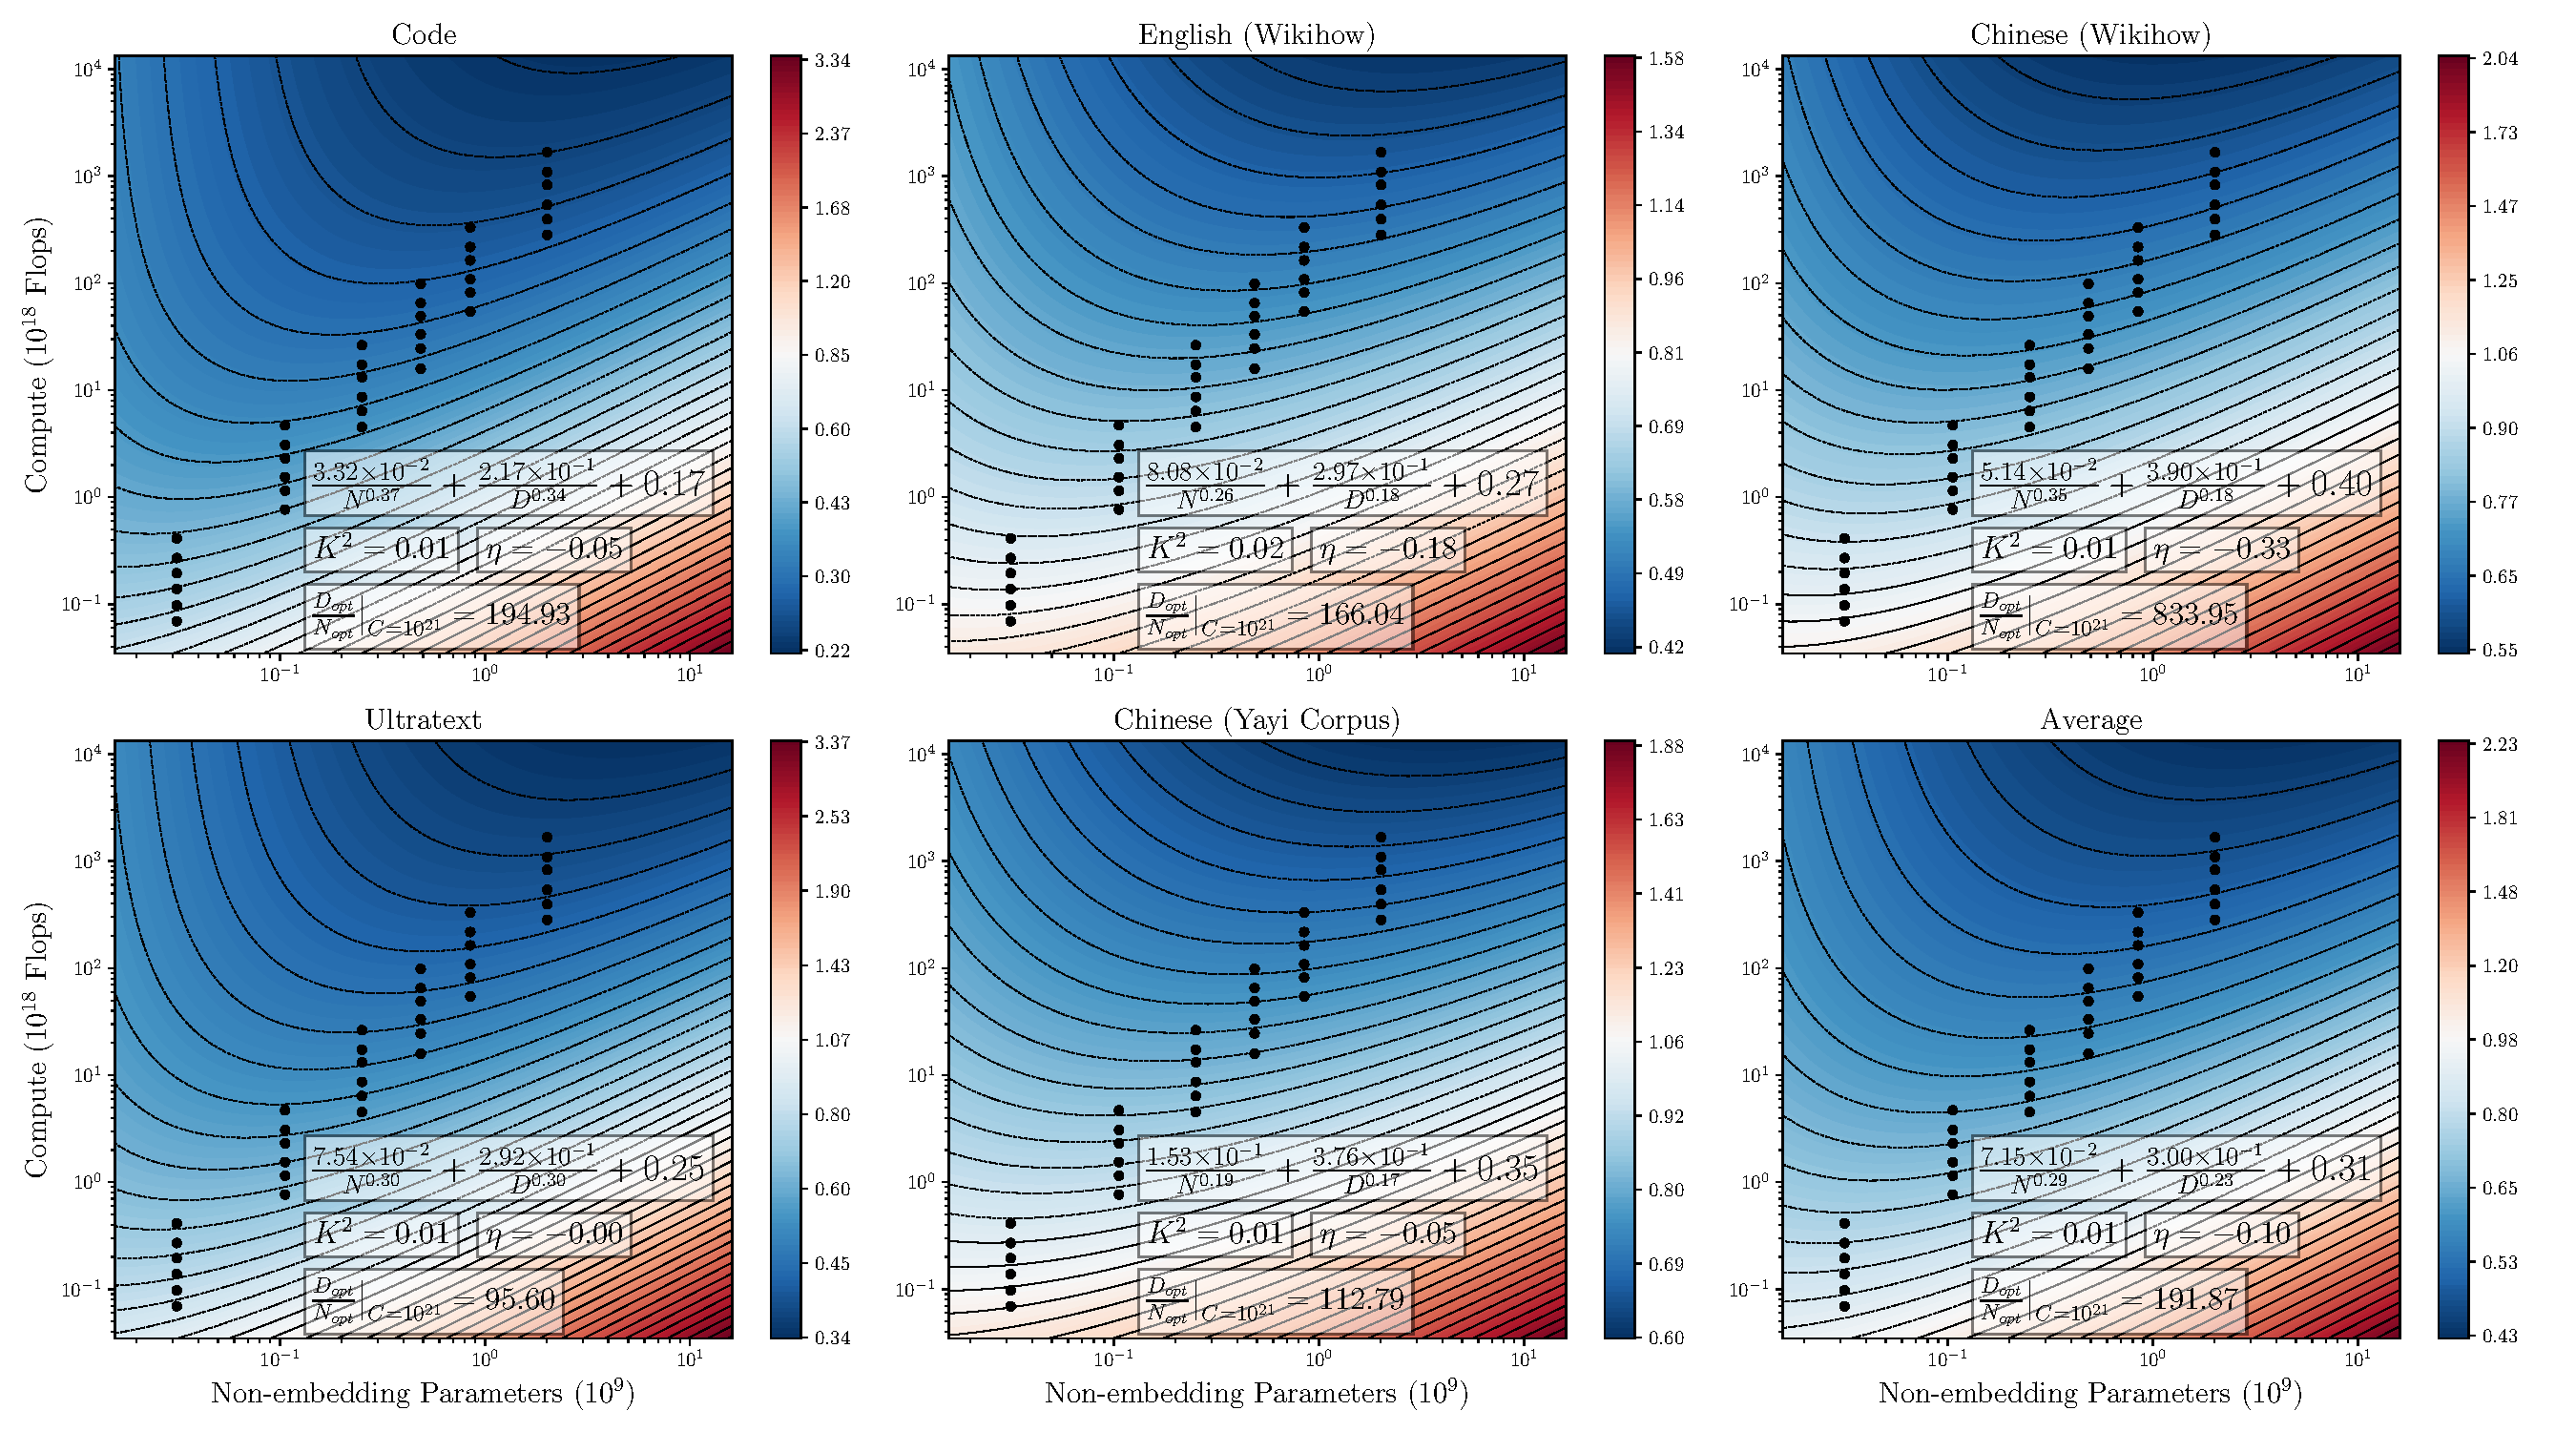
\includegraphics[width=1.0\textwidth]{minicpmFig/wsd_optimal_scaling_law.pdf}
    \caption{使用WSD调度器进行缩放实验的拟合结果。水平线上的黑点表示相同模型规模下不同计算量中的衰减检查点。图例中的$C$为语义完整以Flops为单位表示,未使用EFlops单位。y轴上的$C$以EFlops为单位。}
    \label{fig:wsd_optimalscalinglaw}
\end{figure}



\section{Llama2数据与模型比率的分析}
如\ref{scalinglawwsdlrs}节所述,我们基于Llama2的训练损失曲线分析其数据与模型比率。提取的损失绘制在图\ref{fig:llamascaling}的左侧。我们将x轴转换为计算量Flops,以便在图的右侧比较计算最优区域。

\begin{figure}
    \centering
    \includegraphics[width=1.0\textwidth]{minicpmFig/llama2_scaling.pdf}
    \caption{我们从Llama2论文中提取训练损失数据(左图部分),并使用右图部分估计其论文中的计算最优$\frac{D_{opt}}{N_{opt}}$。绘制的直线是假设使用WSD调度器来估计最优损失包络线。}
    \label{fig:llamascaling}
\end{figure}
